\chapter{Statistické techniky komprese}
\label{kapitolaStatistickaKomprese}
Statistické kompresní metody využívají znalosti tzv. pravděpodobnostního modelu komprimovaných dat. Modelem může být například četnost výskytu jednotlivých symbolů v~textu. Účinnost komprese je závislá na schopnosti co nejpřesněji modelovat zpracovávaná data. Čím více se model přibližuje realitě, tím je účinnost komprese vyšší a naopak.

\section{Pravděpodobnostní model}
\label{pravdepodobnostniModel}
Pravděpodobnostní model přiřazuje pravděpodobnosti výskytu symbolům ve zdrojové zprávě. Na tomto základě například Huffmanovo kódování (viz \ref{huffmanovoKodovani} a \ref{adaptivniHuffman}) přiřazuje symbolům, které se v datech objevují častěji (mají vyšší pravděpodobnost výskytu), kratší kódová slova.

Podle toho, jakým způsobem model vzniká, ho můžeme označit jako statický, semiadaptivní, nebo adaptivní.

\subsection{Statický model}
Tento model je definován při implementaci kompresní metody a při použití se již nijak nemění. Výhodou je rychlost a jednoduchost vytvoření modelu. Například v případě, že budeme zpracovávat výstup pouze jednoho známého zdroje, se tímto způsobem vyhneme opakovanému vytváření modelu, které by vedlo ke stejným, nebo alespoň velmi podobným výsledkům. V opačném případě ale model nemusí datům vůbec odpovídat, čímž bude dosažená účinnost komprese velice nízká.

\subsection{Semiadaptivní model}
Komprimovaná data jsou jedním průchodem statisticky zpracována a následně je vytvořen odpovídající model. K samotné kompresi je ale nutný ještě druhý průchod daty s již vytvořeným modelem. Aby bylo možné data dekomprimovat, je nutné připojit model k~datům. Model je sice přesný, ale velikost zkomprimované zprávy je větší o model. Navíc přístup s dvěma průchody daty činí tyto algoritmy neefektivními a v praxi se moc nepoužívají.

\subsection{Adaptivní model}
Tento model vzniká v průběhu zpracování dat a je postupně aktualizován. To platí i~pro dekompresní algoritmus, ten vytváří model stejně jako kompresní algoritmus z části textu, kterou již dekomprimoval. Díky tomu není nutné model připojovat k datům a také procházet data dvakrát.

\section{Semiadaptivní Huffmanovo kódování}
\label{huffmanovoKodovani}
Huffmanovo kódování je jednou z nejstarších kompresních technik, kterou publikoval již v~roce 1952 David A. Huffman. Semiadaptivní dvouprůchodová verze byla od svého vzniku podrobena dalšímu výzkumu a postupně vylepšena až na adaptivní. Je založeno na dvou vlastnostech nejkratších prefixových\footnote{Prefix značí několik shodných počátečních znaků různých řetězců.} (jednoznačně dekódovatelných) kódů \cite{introductionToDataCompression}:

\begin{enumerate}
\item Symbolům s vyšší pravděpodobností výskytu jsou přiřazována kratší kódová slova.
\item Dvěma symbolům s nejmenší pravděpodobností výskytu jsou přiřazována kódová slova stejné délky.
\end{enumerate}

Algoritmus nejprve seřadí symboly sestupně podle pravděpodobnosti výskytu a poté z nich v krocích konstruuje strom od listů ke kořeni. V každém kroku jsou vybrány dva symboly s nejmenší pravděpodobností výskytu, z nich je vytvořen nový uzel, který je brán jako symbol s kumulovanou pravděpodobností odpovídající součtu dílčích pravděpodobností. Kroky opakujeme až do vybrání všech symbolů, kdy je kumulovaná pravděpodobnost výskytu rovna 1. Nakonec ohodnotíme hrany vystupující z uzlu vlevo číslem 0 a vpravo číslem 1. Kódová slova získáme čtením stromu od kořene k listům. \cite{dataCompression}, \cite{introductionToDataCompression}

\subsection{Postup kódování a dekódování zprávy}
Při kódování zprávy zapisujeme na výstup kódová slova odpovídající čteným symbolům. Naopak při dekódování procházíme strom od uzlu k listům tak, jak jsou čteny jednotlivé znaky kódových slov. Pokud dojdeme do listu, přečetli jsme jeden původní symbol a~můžeme jej vypsat.

\subsection{Vzorový příklad}
Postup lze nejlépe prezentovat na příkladu. Mějme za úkol zakódvat zprávu \uv{MISSISSIPPI} pomocí semiadaptivního Huffmanova kódování. Výsledný strom je zobrazen na obrázku \ref{semiHuffmanStrom} a je sestaven dle návodu popsaného v úvodu této podkapitoly. Místo pravdě\-po\-do\-bno\-stí výskytu jsou použity absolutní četnosti symbolů v listech a kumulativní četnosti v dalších uzlech. Získaná kódová slova pro jednotlivé symboly jsou zobrazena v~tabulce \ref{semiHuffmanStrom}.

\subsubsection{Data po zakódování}
Zakódovaná zpráva je tvaru \texttt{111|0|10|10|0|10|10|0|110|110|0}, kde je znak \uv{\texttt{|}} použit jako oddělovač jednotlivých kódových slov.

\begin{figure}[!htb]
\centering
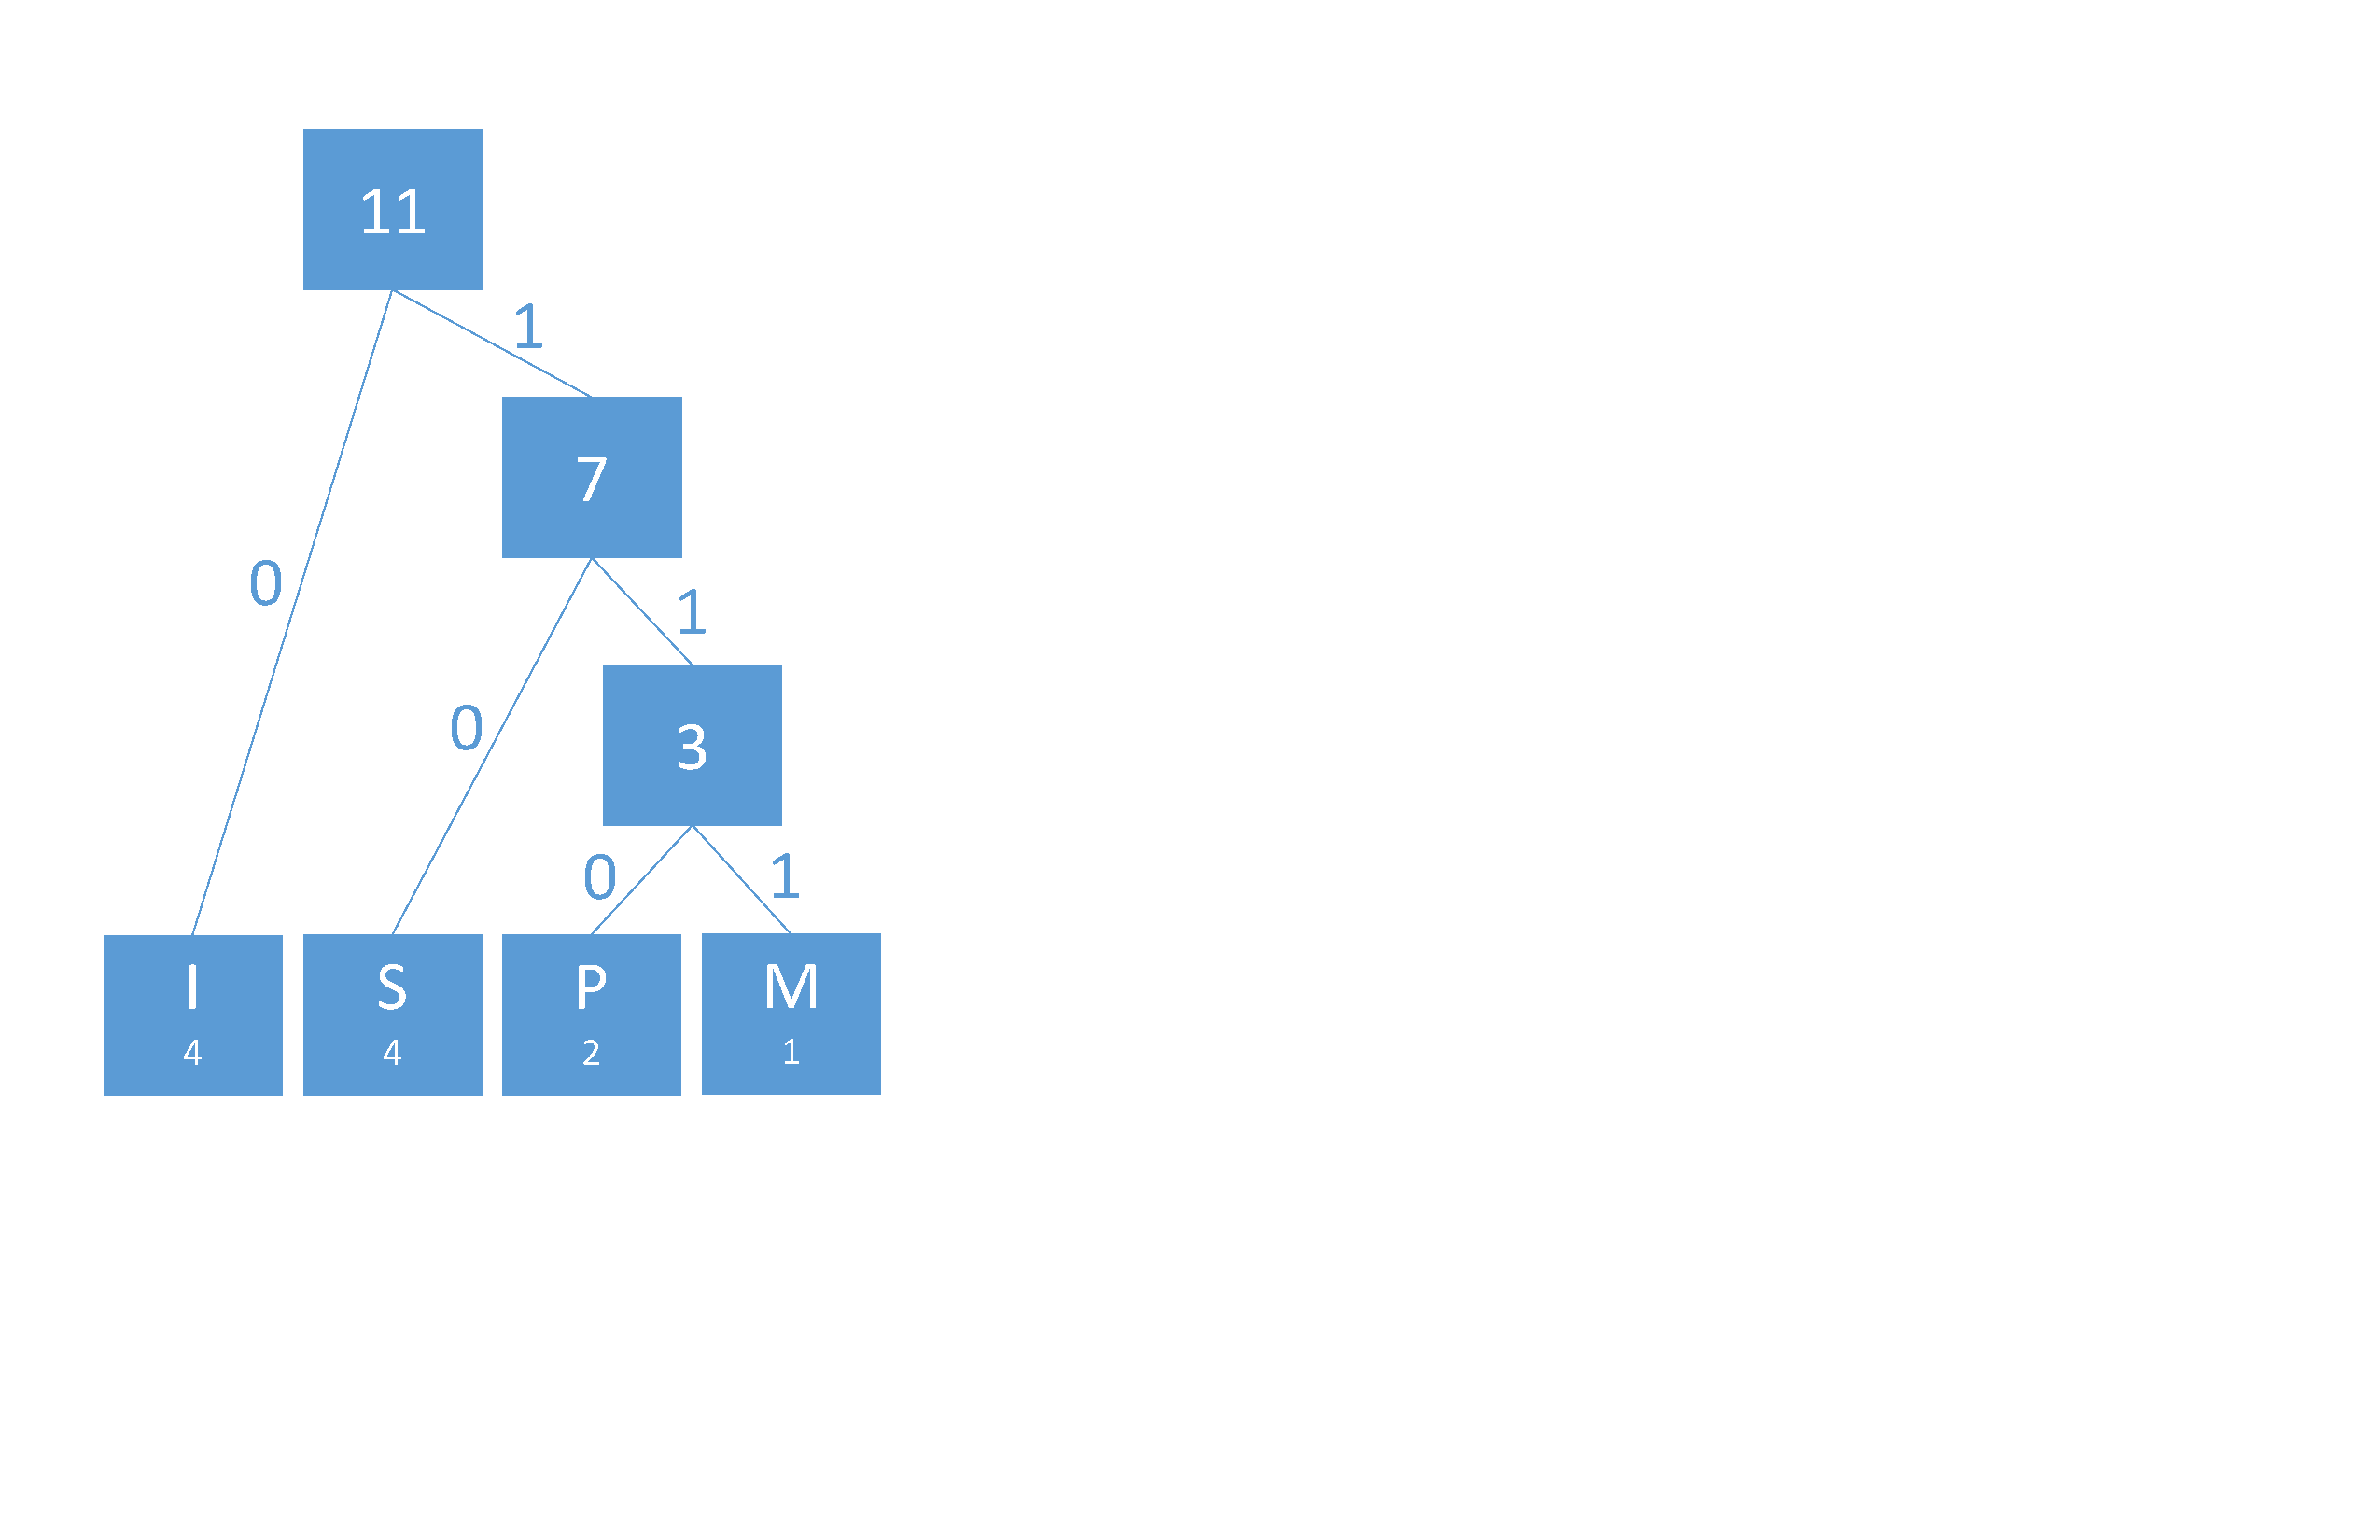
\includegraphics[trim=50 220 770 60, clip, angle=0, width=55mm]{semiHuffman}
\caption{Strom vytvořený při semiadaptivním Huffmanově kódování}
\label{semiHuffmanStrom}
\end{figure}

\begin{table}[!htb]
\centering
\begin{tabular}{|c|c|l|}
\hline
Zdrojový znak & Četnost výskytu & Kódové slovo\\
\hline
I & 4 & 0\\
S & 4 & 10\\
P & 2 & 110\\
M & 1 & 111\\
\hline
\end{tabular}
\caption{Kódová slova semiadaptivního Huffmanova kódu}
\label{semiHuffmanTabulka}
\end{table}

\section{Adaptivní Huffmanovo kódování}
\label{adaptivniHuffman}
Adaptivní Huffmanovo kódování konstruuje strom při kompresi i dekompresi posloupností stejných kroků, tzv. mirroring. Strom je v každém kroku upraven tak, aby produkoval nejkratší kód pro do té doby zpracovanou část dat. Jak se strom mění, mění se i kódy přiřazené jednotlivým symbolům. Listy stromu obsahují symboly a jejich četnosti výskytu, vnitřní uzly obsahují kumulovanou četnost svých potomků.

Implementovaných verzí existuje několik. Níže je představena verze, kterou navrhl Jeffrey S. Vitter a ve které všechny uzly navíc obsahují pořadové číslo, které je využito při rozhodování při aktualizaci stromu. Nejvyšší pořadové číslo $n$ určíme ze vztahu $n = 2m -1$, kde $m$ je počet znaků zdrojové abecedy. Také se zde využívají tzv. bloky -- množiny uzlů se stejnou četností. Způsob kódování a dekódování zprávy je popsán v části \ref{prikladAdaptivniHuffman}.

Algoritmus začíná pouze s uzlem označeným NYT (not yet transmitted), který symbolizuje všechny znaky, které se zatím ve stromu nevyskytují. Je-li ke zpracování načten symbol, který se ještě ve stromě nevyskytuje, je do výstupu vypsáno kódové slovo uzlu NYT následované nezakódovaným a dohodnutým tvarem zpracovávaného symbolu. Následně se z uzlu NYT stane vnitřní uzel a jsou mu přiřazeni dva noví potomci: nový uzel NYT a list reprezentující právě zpracovávaný znak. Poté je strom aktualizován. Je-li ke zpracování načten ve stromě již obsažený symbol, je na výstup vypsáno pouze kódové slovo tohoto symbolu a strom je aktualizován.

Nezakódovaný tvar zpracovávaného symbolu může být například jeho osmibitový ASCII kód. Má-li zdrojová abeceda $\{a_1, a_2, \ldots, a_m\}$ počet znaků roven $m$, pak zvolíme $e,r$ tak, aby splňovala $m= 2^e + r$ a $0 \leq r < 2^e$. Znak $a_k$ poté kódujeme jako $(e+1)$-bitovou reprezentaci čísla $k-1$, je-li $1 \leq k \leq 2r$, jinak je $a_k$ kódován jako $e$-bitová reprezentace čísla $k-r-1$. \cite{dataCompression}, \cite{introductionToDataCompression}

\subsection{Vzorový příklad}
\label{prikladAdaptivniHuffman}
Pokusme se znovu zakódovat slovo MISSISSIPPI a uvažujme anglickou abecedu jako zdrojovou. Ta má 26 znaků, tedy $m=26$, $e = 4$ a $r=10$ a znaky číslujeme $a_1 = \mathrm{A}$ atd.

\subsubsection{Zakódování zprávy a vytvoření stromu}
Začínáme se stromem, který obsahuje pouze kořen NYT. Čteme znak M a na výstup zapíšeme jeho pětibitový nezakódovaný tvar pro $k=13$, tedy \texttt{01100}. Aktualizujeme strom. Čteme znak I, který se ve stromě také nevyskytuje. Na výstup zapíšeme kód uzlu NYT (nyní je to \texttt{0}) a pětibitový nezakódovaný tvar pro $k=9$, tedy \texttt{01000}. Aktualizujeme strom. Dále čteme nový znak S. Na výstup zapíšeme kód uzlu NYT (nyní je to \texttt{00}) a pětibitový nezakódovaný tvar pro $k=19$, tedy \texttt{10010}. Aktualizujeme strom. Dále čteme znak S, který ve stromu již je a tedy vypíšeme pouze jeho kód. Aktualizujeme strom. A tak pokračujeme pro všechny znaky slova. Výsledný strom je zobrazen na obrázku \ref{adaptivniHuffmanStrom}.

\begin{figure}[!htb]
\centering
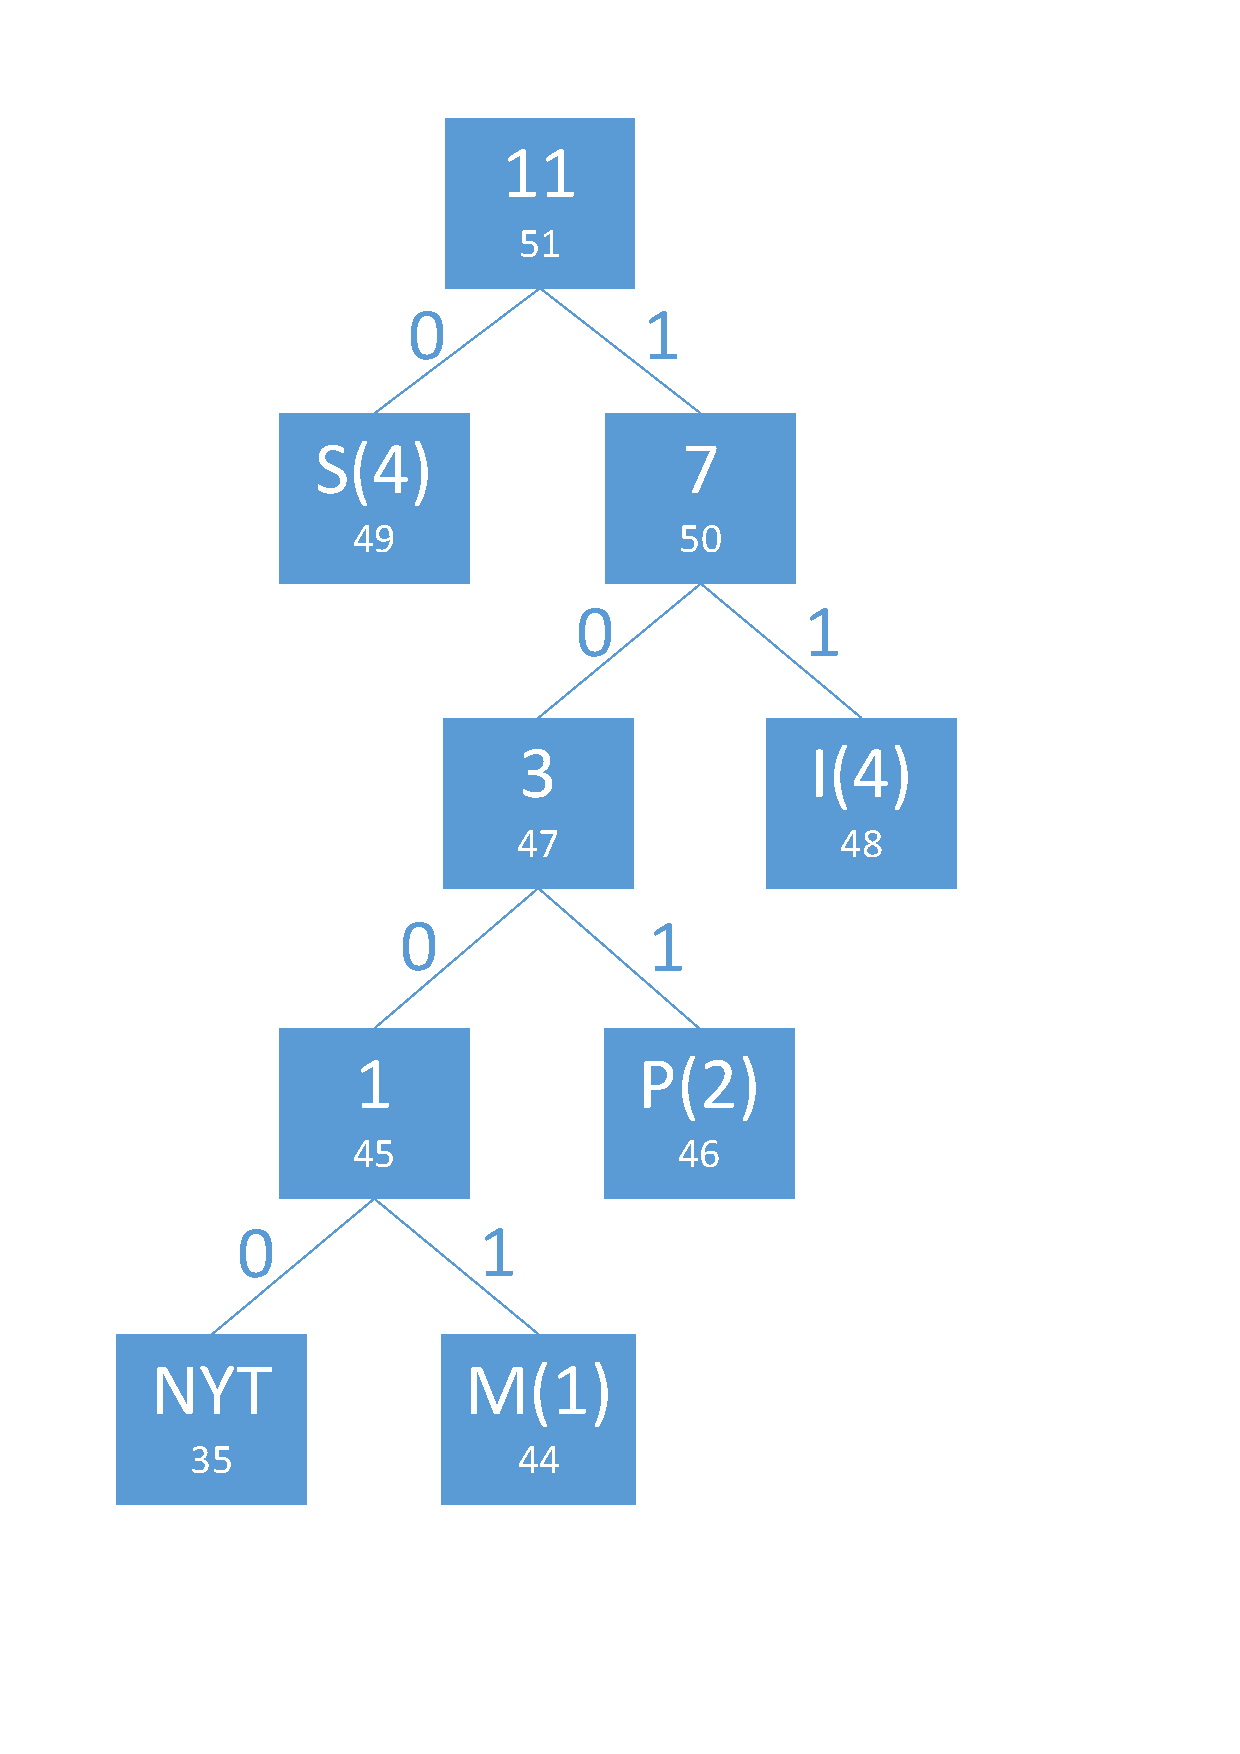
\includegraphics[trim=50 105 130 50, clip, angle=0, width=55mm]{adaptHuffman}
\caption{Strom vytvořený při adaptivním Huffmanově kódování}
\label{adaptivniHuffmanStrom}
\end{figure}

\subsubsection{Zakódovaná zpráva}
Výsledná zakódovaná zpráva je tvaru \texttt{01100|0|01000|00|10010|101|11|0|1|01|000|\\01111|1001|11}, kde jsem pro přehlednost vložil oddělovač \uv{\texttt{|}} oddělující jednotlivé vý\-zna\-mné bloky.

\subsubsection{Dekódování zprávy}
Přečteme $e=4$ bitům znaků, jejichž hodnota jakožto čtyřbitového čísla je 6, což je menší než $r=10$. Přečteme další znak, hodnota tohoto pětibitového čísla je 12 a tedy jsme přečetli symbol $a_{13} = \mathrm{M}$. Aktualizujeme strom. Následuje 0, která je kódovým slovem pro uzel NYT, po něm vždy následuje nezakódovaný symbol. Obdobně jako pro M přečteme symbol $a_8 = \mathrm{I}$. Aktualizujeme strom. Následuje kódové slovo uzlu NYT a~symbol \mbox{$a_{19} = \mathrm{S}$}. Dále čteme kódové slovo uzlu pro symbol S. Takto pokračujeme, dokud nepřečteme všechna slova zakódované zprávy.